\documentclass[12pt,a4paper]{book}
\usepackage[utf8]{inputenc}
\usepackage[english]{babel}
\usepackage{amsmath}
\usepackage{amsfonts}
\usepackage{amssymb}
\author{Mihai Cornel}
\title{Python Tkinter}

\usepackage{graphicx} 
\usepackage{listings}

\begin{document}
\section{Ce este Tkiner?}
	Tkinter este un modul Python pentru crearea interfețelor grafice(GUI) și este inclus în toate distribuțiile standard Python. Acest modul oferă o interfață pentru setul de instrumente Tk și funcționează pe modelul orientat obiect. Setul de instrumente Tk este o colecție multiplatformă de elemente de control grafic, cunoscute sub numele de widget-uri, pentru construirea interfețelor grafice.

Pentru verificarea versiunii Tcl/Tk în terminal introduceți:
\begin{verbatim}
$ tclsh
% info patchlevel
	8.6.10
\end{verbatim}

Pentru a verifica instalarea corectă a modulului Tkinter în terminal introduceți comanda:

\begin{verbatim}
$ python3 -m tkinter
\end{verbatim}

Această comanda deschide următoarea fereastră:

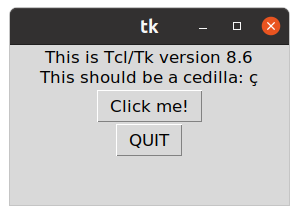
\includegraphics[width=\linewidth]{/home/mhcrnl/Desktop/Blog/img02.png}

Acest modul oferă utilizatorilor Python o modalitate simplă de a crea elemente grafice folosind widgeturile găsite în setul de instrumente Tk.  Widget-urile Tk pot fi folosite pentru a construi butoane, meniuri, câmpuri de date etc. într-o aplicație Python.  Odată create, aceste elemente grafice pot fi asociate sau pot interacționa cu caracteristici, funcționalitați, metode, date sau chiar alte widgeturi. 

De exemplu, un widget de buton poate accepta clicuri de mouse și poate fi, de asemenea, programat pentru a efectua un fel de acțiune, cum ar fi ieșirea din aplicație.

Aceasta este un program Python cu Tkinter și rezultatul după rularea programului:
\lstinputlisting[language=Python, frame=single]{main01.py}
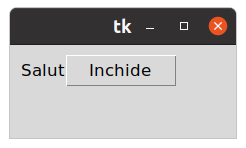
\includegraphics[width=\linewidth]{img01.png}

\begin{lstlisting}
print("hello")
\end{lstlisting}

\lstinputlisting[language=Python]{/home/mhcrnl/Desktop/Blog/oct2021/pyart04/main.py}


    
\begin{verbatim}
  print(“Hello, World!”) 
\end{verbatim} 


   

	



  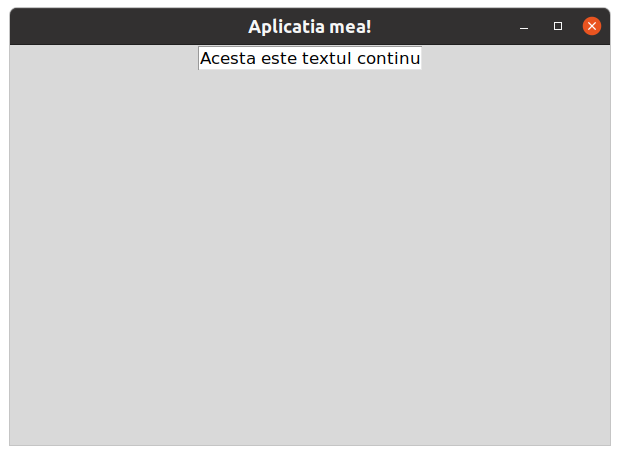
\includegraphics[width=\linewidth]{/home/mhcrnl/Desktop/Blog/oct2021/pyart04/img01.png}
  
 






\end{document}
